%%%%%%%%%%%%%%%%%%%%%%%%%%%%%%%%%%%%%%%%%%%%%%%%%%%%%%%%%%%%%%%%%%%%%%%%%%%%%%
% SECTION : Différents algorithmes de détection
%%%%%%%%%%%%%%%%%%%%%%%%%%%%%%%%%%%%%%%%%%%%%%%%%%%%%%%%%%%%%%%%%%%%%%%%%%%%%%

\subsection{Différents algorithmes de détection}

%%%%%%%%%%%%%%%%%%%%%%%%%%%%%%%%%%%%%%%%%%%%%%%%%%%%%%%%%%%%%%%%%%%%%%%%%%%%%%
% Sous-section : Principe du CA-CFAR
%%%%%%%%%%%%%%%%%%%%%%%%%%%%%%%%%%%%%%%%%%%%%%%%%%%%%%%%%%%%%%%%%%%%%%%%%%%%%%

\subsubsection{Principe du CA-CFAR }

La détection CFAR (Constant False Alarm Rate) correspond à une approche adaptative utilisée dans les radars pour distinguer les retours d’une cible d’un bruit de fond important ou d’interférences. Le principe de cet algorithme consiste à tester une cellule (Cell Under Test : CUT) afin de déterminer si une cible est présente ou s’il s’agit simplement de bruit.  
Pour cela, le niveau du bruit de fond est estimé à partir des cellules adjacentes à la CUT, appelées Cellules de Références (Reference Cells : RC). Les cellules immédiatement voisines, susceptibles d’être influencées par la puissance de la CUT, sont exclues du calcul : ce sont les Guard Cells.  
Une cible est considérée comme présente si la puissance mesurée dans la CUT est supérieure à la fois aux cellules voisines et au niveau moyen estimé.

\begin{figure}[h]
    \centering
    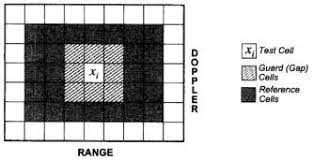
\includegraphics[width=0.6\textwidth]{src/rapport_complet/img/cellule_CFAR.jpg}
    \caption{Cellule de détection CFAR}
    \label{fig:image_radar_CFAR}
\end{figure}

%%%%%%%%%%%%%%%%%%%%%%%%%%%%%%%%%%%%%%%%%%%%%%%%%%%%%%%%%%%%%%%%%%%%%%%%%%%%%%
% Schéma CFAR en TikZ
%%%%%%%%%%%%%%%%%%%%%%%%%%%%%%%%%%%%%%%%%%%%%%%%%%%%%%%%%%%%%%%%%%%%%%%%%%%%%%

\begin{figure}[h!]
\centering
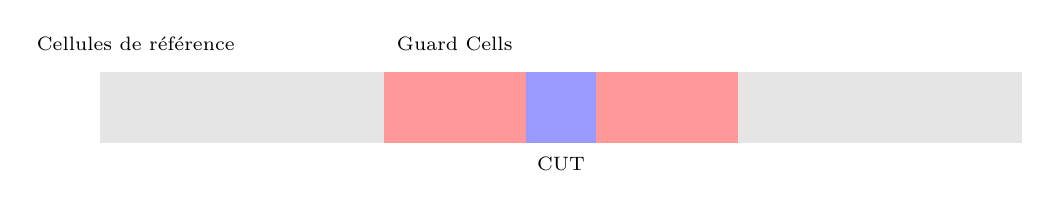
\begin{tikzpicture}[scale=0.9]
\foreach \x in {-6,...,6}{
  \ifnum\x=-6
    \fill[gray!20] (\x,0) rectangle ++(1,1);
  \else\ifnum\x=-5
    \fill[gray!20] (\x,0) rectangle ++(1,1);
  \else\ifnum\x=-4
    \fill[gray!20] (\x,0) rectangle ++(1,1);
  \else\ifnum\x=-3
    \fill[gray!20] (\x,0) rectangle ++(1,1);
  \else\ifnum\x=-2
    \fill[red!40] (\x,0) rectangle ++(1,1);
  \else\ifnum\x=-1
    \fill[red!40] (\x,0) rectangle ++(1,1);
  \else\ifnum\x=0
    \fill[blue!40] (\x,0) rectangle ++(1,1);
  \else\ifnum\x=1
    \fill[red!40] (\x,0) rectangle ++(1,1);
  \else\ifnum\x=2
    \fill[red!40] (\x,0) rectangle ++(1,1);
  \else\ifnum\x=3
    \fill[gray!20] (\x,0) rectangle ++(1,1);
  \else
    \fill[gray!20] (\x,0) rectangle ++(1,1);
  \fi\fi\fi\fi\fi\fi\fi\fi\fi\fi
}
\node at (-5.5,1.4) {\scriptsize Cellules de référence};
\node at (-1,1.4) {\scriptsize Guard Cells};
\node at (0.5,-0.3) {\scriptsize CUT};
\end{tikzpicture}
\caption{Disposition typique des cellules dans un schéma CFAR}
\label{fig:cellules_CFAR}
\end{figure}

%%%%%%%%%%%%%%%%%%%%%%%%%%%%%%%%%%%%%%%%%%%%%%%%%%%%%%%%%%%%%%%%%%%%%%%%%%%%%%
% Estimation du bruit
%%%%%%%%%%%%%%%%%%%%%%%%%%%%%%%%%%%%%%%%%%%%%%%%%%%%%%%%%%%%%%%%%%%%%%%%%%%%%%

Le niveau du clutter (fouillis radar, échos parasites) est estimé par la moyenne arithmétique des échantillons contenus dans la fenêtre de référence \cite{fstech_chapitre5_cfar} :
\begin{equation}
Q = \frac{1}{M} \sum_{i=1}^{M} x_i,
\end{equation}
où $Q$ représente l’estimation du niveau moyen du clutter, $M$ le nombre de cellules de référence, et $x_i$ la puissance mesurée dans la $i^{\text{ème}}$ cellule.

En détection quadratique, la fonction de densité de probabilité (FDP) de la variable $X$ à la sortie du détecteur suit une loi exponentielle :
\begin{equation}
f_X(x) = \frac{1}{2\sigma^2} e^{-x / 2\sigma^2}, \quad x \ge 0.
\end{equation}

%%%%%%%%%%%%%%%%%%%%%%%%%%%%%%%%%%%%%%%%%%%%%%%%%%%%%%%%%%%%%%%%%%%%%%%%%%%%%%
% Seuil de détection
%%%%%%%%%%%%%%%%%%%%%%%%%%%%%%%%%%%%%%%%%%%%%%%%%%%%%%%%%%%%%%%%%%%%%%%%%%%%%%

Le seuil de détection, dit adaptatif, correspond au niveau à partir duquel une cible est estimée présente :
\begin{equation}
T = \alpha Q.
\end{equation}

%%%%%%%%%%%%%%%%%%%%%%%%%%%%%%%%%%%%%%%%%%%%%%%%%%%%%%%%%%%%%%%%%%%%%%%%%%%%%%
% Probabilités de détection et de fausse alarme
%%%%%%%%%%%%%%%%%%%%%%%%%%%%%%%%%%%%%%%%%%%%%%%%%%%%%%%%%%%%%%%%%%%%%%%%%%%%%%

La probabilité de fausse alarme $P_{fa}$ désigne la probabilité qu’une mesure dépasse le seuil $T$ alors qu’aucune cible n’est présente :
\begin{equation}
P_{fa} = P(X > T \,|\, H_0),
\end{equation}
tandis que la probabilité de détection $P_d$ représente la probabilité qu’une mesure dépasse ce seuil lorsqu’une cible est effectivement présente :
\begin{equation}
P_d = P(X > T \,|\, H_1).
\end{equation}

%%%%%%%%%%%%%%%%%%%%%%%%%%%%%%%%%%%%%%%%%%%%%%%%%%%%%%%%%%%%%%%%%%%%%%%%%%%%%%
% Détection déterministe
%%%%%%%%%%%%%%%%%%%%%%%%%%%%%%%%%%%%%%%%%%%%%%%%%%%%%%%%%%%%%%%%%%%%%%%%%%%%%%

\subsection{Détection CFAR déterministe}

Sous l’hypothèse d’un clutter gaussien complexe centré, les composantes $I$ et $Q$ sont gaussiennes indépendantes de variance $\sigma^2$.  
La puissance $X = I^2 + Q^2$ suit une loi exponentielle :
\begin{equation}
f_X(x) = \frac{1}{2\sigma^2} e^{-x / 2\sigma^2}, \quad x \ge 0.
\end{equation}

La probabilité de fausse alarme s’écrit :
\begin{equation}
P_{fa} = \left( 1 + \frac{\alpha}{M} \right)^{-M},
\end{equation}
et le facteur de seuil associé :
\begin{equation}
\alpha = M \left( P_{fa}^{-1/M} - 1 \right).
\end{equation}

Sous l’hypothèse $H_1$, la présence d’une cible augmente la moyenne de la loi exponentielle d’un facteur $(1+\mathrm{SNR})$ :
\begin{equation}
P_d = \left( 1 + \frac{\alpha}{M(1+\mathrm{SNR})} \right)^{-M}.
\end{equation}

%%%%%%%%%%%%%%%%%%%%%%%%%%%%%%%%%%%%%%%%%%%%%%%%%%%%%%%%%%%%%%%%%%%%%%%%%%%%%%
% Détection non déterministe
%%%%%%%%%%%%%%%%%%%%%%%%%%%%%%%%%%%%%%%%%%%%%%%%%%%%%%%%%%%%%%%%%%%%%%%%%%%%%%

\subsection{Détection CFAR non déterministe}

Dans les environnements réels, le clutter radar n’est pas toujours gaussien : il provient souvent de phénomènes multiplicatifs (texture × speckle).  
Les échos radar sont alors mieux modélisés par d’autres lois statistiques : Rayleigh, $\chi^2$, Rician, K-distribution, ou Weibull.

%%%%%%%%%%%%%%%%%%%%%%%%%%%%%%%%%%%%%%%%%%%%%%%%%%%%%%%%%%%%%%%%%%%%%%%%%%%%%%
% Loi de Rayleigh
%%%%%%%%%%%%%%%%%%%%%%%%%%%%%%%%%%%%%%%%%%%%%%%%%%%%%%%%%%%%%%%%%%%%%%%%%%%%%%

\subsubsection{Loi de Rayleigh}

La loi de Rayleigh est utilisée lorsque le signal radar résulte de la somme de nombreuses composantes aléatoires indépendantes en phase et amplitude, typiques d’un clutter homogène sans composante directe (par exemple : mer calme ou terrain uniforme).  
Elle décrit les amplitudes du signal complexe en absence de cible cohérente :
\begin{equation}
f_A(a)=\frac{a}{\sigma^2} e^{-a^2/2\sigma^2}, \quad a\ge0.
\end{equation}
La détection se fait souvent sur la puissance $A^2$, suivant une loi exponentielle :
\begin{equation}
f_X(x) = \frac{1}{2\sigma^2} e^{-x/2\sigma^2}.
\end{equation}
Les probabilités associées sont alors :
\begin{equation}
P_{fa} = \left(1+\frac{\alpha}{M}\right)^{-M},
\end{equation}
\begin{equation}
P_d = \left(1+\frac{\alpha}{M(1+\mathrm{SNR})}\right)^{-M},
\end{equation}
ce qui correspond au modèle CFAR exponentiel classique \cite{skolnik2001, richards2005}.  
Ce modèle repose sur l’hypothèse d’un clutter homogène, d’un bruit gaussien centré sans composante cohérente, et correspond à un modèle déterministe de variance fixe.

%%%%%%%%%%%%%%%%%%%%%%%%%%%%%%%%%%%%%%%%%%%%%%%%%%%%%%%%%%%%%%%%%%%%%%%%%%%%%%
% Loi Chi² / Gamma
%%%%%%%%%%%%%%%%%%%%%%%%%%%%%%%%%%%%%%%%%%%%%%%%%%%%%%%%%%%%%%%%%%%%%%%%%%%%%%

\subsubsection{Loi $\chi^2$ / Gamma}

La loi $\chi^2$ ou Gamma est utilisée lorsque le signal est issu d’un moyennage incohérent de plusieurs looks indépendants, ce qui augmente les degrés de liberté et réduit le speckle (cas d’imagerie SAR multi-look).  
La densité est donnée par :
\begin{equation}
f_X(x)=\frac{1}{2^{k/2}\Gamma(k/2)}x^{k/2-1}e^{-x/2}.
\end{equation}
Les probabilités $P_{fa}$ et $P_d$ s’expriment sous forme d’intégrales de fonctions Gamma incomplètes \cite{richards2005, skolnik2001} :
\begin{equation}
P_{fa} = \int_{\alpha Q}^{\infty} f_X(x|H_0) dx, \quad
\end{equation}
\begin{equation}
P_d = \int_{\alpha Q}^{\infty} f_X(x|H_1) dx.
\end{equation}
Ces intégrales sont généralement évaluées numériquement.  
Ce modèle repose sur une hypothèse de multi-look homogène et demeure déterministe pour des paramètres $k$ connus.

%%%%%%%%%%%%%%%%%%%%%%%%%%%%%%%%%%%%%%%%%%%%%%%%%%%%%%%%%%%%%%%%%%%%%%%%%%%%%%
% Loi de Rice
%%%%%%%%%%%%%%%%%%%%%%%%%%%%%%%%%%%%%%%%%%%%%%%%%%%%%%%%%%%%%%%%%%%%%%%%%%%%%%

\subsubsection{Loi de Rice}

La loi de Rice est adaptée à la présence d’une composante cohérente dans un fond gaussien diffus (par ex. un bateau sur mer calme).  
Elle décrit l’amplitude d’un signal comprenant une partie déterministe (la cible) et un bruit gaussien :
\begin{equation}
f_A(a)=\frac{a}{\sigma^2}\exp\!\Big(-\frac{a^2+s^2}{2\sigma^2}\Big)I_0\!\Big(\frac{a s}{\sigma^2}\Big).
\end{equation}
La probabilité de détection associée s’écrit \cite{skolnik2001, richards2005} :
\begin{equation}
P_d = Q_1\!\left(\frac{s}{\sigma},\frac{T}{\sigma}\right),
\end{equation}
où $Q_1$ est la fonction de Marcum.  
Le seuil $T = \alpha Q$ est fixé à partir d’un $P_{fa}$ donné selon la loi du clutter.  
Ce modèle est non déterministe : la cible est aléatoire sur un fond gaussien centré.

%%%%%%%%%%%%%%%%%%%%%%%%%%%%%%%%%%%%%%%%%%%%%%%%%%%%%%%%%%%%%%%%%%%%%%%%%%%%%%
% Loi K
%%%%%%%%%%%%%%%%%%%%%%%%%%%%%%%%%%%%%%%%%%%%%%%%%%%%%%%%%%%%%%%%%%%%%%%%%%%%%%

\subsubsection{Loi K}

La loi K modélise le clutter non gaussien à texture, caractéristique des images SAR haute résolution (mer agitée, zones urbaines).  
Elle correspond à un produit aléatoire $X = S \times Y$, où $S$ suit une loi Gamma (texture lente) et $Y$ une loi $\chi^2$ (speckle rapide) :
\begin{equation}
f_X(x)=\frac{2}{\Gamma(\nu)}\left(\frac{\nu}{\mu}\right)^{\nu/2} x^{(\nu-2)/2} K_{\nu-2}\!\Big(2\sqrt{\frac{\nu x}{\mu}}\Big).
\end{equation}
Aucune solution analytique simple n’existe pour $P_{fa}$ et $P_d$, qui sont estimés numériquement ou par Monte-Carlo \cite{habib2008, schukin2008}.  
Ce modèle non déterministe rend compte des fortes variations de texture et de la nature multiplicative du clutter radar. Il est fréquemment utilisé dans des contextes d'imagerie SAR haute résolution (mer agitée, zones urbaines).

%%%%%%%%%%%%%%%%%%%%%%%%%%%%%%%%%%%%%%%%%%%%%%%%%%%%%%%%%%%%%%%%%%%%%%%%%%%%%%
% Loi de Weibull
%%%%%%%%%%%%%%%%%%%%%%%%%%%%%%%%%%%%%%%%%%%%%%%%%%%%%%%%%%%%%%%%%%%%%%%%%%%%%%

\subsubsection{Loi de Weibull}

La loi de Weibull s’applique à des environnements terrestres ou littoraux où la distribution du clutter présente des queues variables selon un paramètre de forme $k$ :
\begin{equation}
f_X(x)=\frac{k}{\lambda}\Big(\frac{x}{\lambda}\Big)^{k-1}\exp\!\Big[-\Big(\frac{x}{\lambda}\Big)^k\Big].
\end{equation}
La probabilité de fausse alarme correspondante est donnée par \cite{el_darymli2018, skolnik2001} :
\begin{equation}
P_{fa} = \exp\!\Big[-\Big(\frac{T}{\lambda}\Big)^k\Big].
\end{equation}
Le seuil $T = \alpha Q$ est ajusté localement sur les données, et les probabilités de détection sont obtenues par simulation.  
Ce modèle non déterministe décrit un clutter modérément hétérogène avec des paramètres $(k, \lambda)$ estimés localement.

%%%%%%%%%%%%%%%%%%%%%%%%%%%%%%%%%%%%%%%%%%%%%%%%%%%%%%%%%%%%%%%%%%%%%%%%%%%%%%
% Tableau et conclusion 
%%%%%%%%%%%%%%%%%%%%%%%%%%%%%%%%%%%%%%%%%%%%%%%%%%%%%%%%%%%%%%%%%%%%%%%%%%%%%%



\subsection{Méthodes CFAR adaptées à l’imagerie SAR}

En imagerie SAR, le choix du détecteur CFAR dépend fortement de la nature du clutter et de la résolution.  
Les modèles déterministes (exponentiel, Rayleigh) sont performants dans les zones homogènes où les hypothèses d’indépendance et de moyenne constante du bruit sont respectées.  
Cependant, dans des environnements réels complexes, ces hypothèses sont souvent faussées, notamment en milieu côtier ou urbain où la texture du clutter varie fortement.  
C’est pourquoi les approches non déterministes (K-distribution, Weibull, NG) sont généralement préférées.

Le détecteur CA-CFAR classique reste la référence en milieu homogène pour sa simplicité et sa formulation analytique.  
Mais son efficacité diminue dans les régions hétérogènes ou en présence de cibles multiples.  
Des variantes ont donc été introduites :  
l’OS-CFAR (Order Statistic), qui sélectionne la $k$-ième valeur parmi les cellules de référence pour résister aux valeurs aberrantes,  
Le GO/SO-CFAR (Greatest/Smallest Of), utilisé pour compenser les bords ou gradients de clutter,  
et le ML-CFAR (Maximum Likelihood CFAR), qui ajuste le seuil en estimant la densité réelle du clutter, souvent sous loi K ou NG \cite{habib2008}.  

Plus récemment, des approches hybrides CFAR–apprentissage profond ont émergé \cite{yang2024}.  
Elles consistent à appliquer un CFAR local pour générer des propositions de détection, ensuite validées ou rejetées par un réseau neuronal (CNN).  
Ces méthodes offrent un excellent compromis entre robustesse statistique et adaptabilité contextuelle, notamment pour la détection de navires sur images SAR à très haute résolution.

Ainsi, le CA-CFAR est optimal pour les mers calmes (clutter exponentiel), l’OS-CFAR s’impose dans les zones hétérogènes, le ML- ou NG-CFAR est recommandé pour des environnements non-gaussiens et les approches hybrides CFAR + CNN sont les plus performantes pour les scènes SAR haute résolution (HR) complexes.

\begin{figure}[h!]
\centering
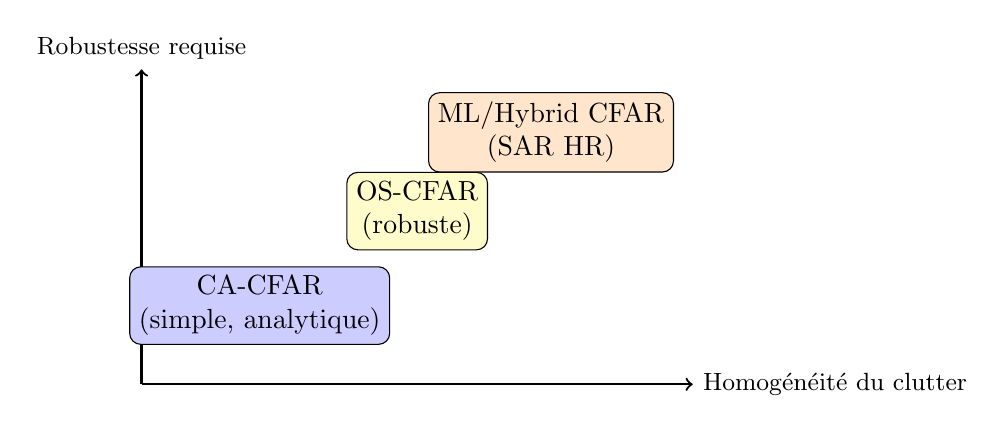
\begin{tikzpicture}
\draw[->,thick] (0,0)--(7,0) node[right]{\small Homogénéité du clutter};
\draw[->,thick] (0,0)--(0,4) node[above]{\small Robustesse requise};
\node[draw,fill=blue!20,rounded corners,align=center] at (1.5,1) {CA-CFAR\\(simple, analytique)};
\node[draw,fill=yellow!20,rounded corners,align=center] at (3.5,2.2) {OS-CFAR\\(robuste)};
\node[draw,fill=orange!20,rounded corners,align=center] at (5.2,3.2) {ML/Hybrid CFAR\\(SAR HR)};
\end{tikzpicture}
\caption{Choix de la méthode CFAR selon le contexte d’imagerie}
\end{figure}

\subsection{Tableau comparatif des lois de clutter}

L’ensemble de ces modèles et méthodes de détection CFAR illustre l’importance d’adapter la stratégie de détection à la nature statistique du clutter.  
Les modèles déterministes, fondés sur des hypothèses de bruit gaussien homogène, offrent des solutions analytiques simples et peu coûteuses en calcul, mais montrent leurs limites dès que la scène radar devient hétérogène ou fortement texturée.  
À l’inverse, les modèles non déterministes, tels que la loi K ou la loi de Weibull, décrivent plus fidèlement les comportements statistiques observés en imagerie SAR haute résolution, au prix d’une complexité de calcul plus élevée et d’une estimation fine des paramètres locaux.

Dans un contexte opérationnel, le compromis entre précision de modélisation, robustesse et charge computationnelle demeure essentiel.  
Ainsi, pour des scènes homogènes, les approches classiques comme le CA-CFAR restent pertinentes, tandis que dans les environnements complexes ou non gaussiens, les méthodes adaptatives (OS-, ML-, NG-CFAR) ou hybrides (CFAR–CNN) constituent aujourd’hui les solutions les plus performantes.  
Ces approches permettent non seulement de maintenir un taux de fausse alarme constant, mais aussi d’améliorer significativement la probabilité de détection dans des contextes d’imagerie réalistes.
\begin{table}[H]
\centering
\begin{tabular}{p{2.5cm}p{2.5cm}p{2.2cm}p{2.2cm}p{2cm}p{2cm}}
\toprule
\textbf{Loi} & \textbf{Hypothèses principales} & \textbf{Type} & \textbf{Méthode de calcul} & \textbf{Complexité} & \textbf{Contextes d’usage} \\
\midrule
Exponentielle & Clutter homogène, indépendantes et identiquement distribuées, mono-look & Déterministe & Formules fermées (Gamma) & $O(1)$ & Milieu marin calme, faible texture \\
Rayleigh & Signal centré, gaussien & Déterministe & Identique à exponentielle (puissance) & $O(1)$ & Bruit d’amplitude homogène \\
$\chi^2$/Gamma & Multi-look, indépendantes et identiquement distribuées & Déterministe & Fonctions Gamma incomplètes & $O(M)$ & Imagerie SAR multi-look \\
Rician & Cible + bruit gaussien & Non-déterministe & Fonction de Marcum $Q_1$ & $O(1)$ (numérique) & Cible cohérente (bateaux, structures) \\
K-distribution & Speckle × texture (clutter non-gaussien) & Non-déterministe & Intégration numérique / Monte-Carlo & $O(N\!M)$ & SAR HR, mer agitée, zones urbaines \\
Weibull & Texture terrestre hétérogène & Non-déterministe & Évaluation directe ou Monte-Carlo & $O(M)$ & Sols, zones littorales \\
\bottomrule
\end{tabular}
\caption{Synthèse des lois de clutter, leurs hypothèses et complexités associées.}
\end{table}



%%%%%%%%%%%%%%%%%%%%%%%%%%%%%%%%%%%%%%%%%%%%%%%%%%%%%%%%%%%%%%%%%%%%%%%%%%%%%%
% SECTION : Fusion de détection
%%%%%%%%%%%%%%%%%%%%%%%%%%%%%%%%%%%%%%%%%%%%%%%%%%%%%%%%%%%%%%%%%%%%%%%%%%%%%%

\subsection{Fusion de détection}

La fusion de détection devient particulièrement pertinente dans un contexte où plusieurs plateformes radar opèrent simultanément et observent une même scène selon des géométries différentes.  
Elle vise à mettre en relation les informations issues de chaque plateforme afin d’exploiter leur complémentarité géométrique et informationnelle, tout en évaluant l’amélioration potentielle de la robustesse de la détection face au bruit et au speckle, inhérents à l’imagerie radar, par rapport à une exploitation indépendante des capteurs.

Dans ce cadre, la \emph{décision} correspond à la sortie de l’algorithme de détection et se formalise par un choix binaire indiquant la présence ou l’absence d’une cible dans la scène observée.  
La combinaison de décisions issues de chaînes de traitement complètes — incluant la formation d’image par des méthodes telles que Range-Doppler ou Back-Projection, suivie d’une modélisation statistique du clutter et d’une détection de type CFAR — permet d’apprécier la cohérence globale du traitement et la stabilité des performances de détection lorsque des hypothèses identiques sont appliquées à des acquisitions issues de points de vue distincts.

%%%%%%%%%%%%%%%%%%%%%%%%%%%%%%%%%%%%%%%%%%%%%%%%%%%%%%%%%%%%%%%%%%%%%%%%%%%%%%
% Sous-section : Niveaux de fusion en imagerie SAR
%%%%%%%%%%%%%%%%%%%%%%%%%%%%%%%%%%%%%%%%%%%%%%%%%%%%%%%%%%%%%%%%%%%%%%%%%%%%%%

\subsubsection{Niveaux de fusion en imagerie SAR}

Dans le cadre de l’imagerie SAR, la fusion peut être envisagée à différents niveaux de la chaîne de traitement.  
Selon le stade auquel les informations sont combinées, la fusion agit sur des grandeurs physiques différentes — signaux complexes, images formées, descripteurs ou décisions — et repose sur des modèles mathématiques distincts \cite{hall1997,llinas2004,varshney1997}.  
Quatre niveaux de fusion sont classiquement distingués : le niveau données, le niveau pixel, le niveau caractéristiques et le niveau décision.

%%%%%%%%%%%%%%%%%%%%%%%%%%%%%%%%%%%%%%%%%%%%%%%%%%%%%%%%%%%%%%%%%%%%%%%%%%%%%%
% Data-level fusion
%%%%%%%%%%%%%%%%%%%%%%%%%%%%%%%%%%%%%%%%%%%%%%%%%%%%%%%%%%%%%%%%%%%%%%%%%%%%%%

\subsubsection{Fusion au niveau données (Data-level fusion)}

La fusion au niveau données correspond à la combinaison directe des signaux radar complexes acquis par les différentes plateformes, avant toute formation d’image.  
Dans un contexte SAR, il s’agit typiquement de fusionner les signaux I/Q après compression en distance, ou directement les échos bruts synchronisés \cite{richards2014}.

D’un point de vue physique, cette approche repose sur la cohérence de phase entre capteurs, ce qui impose une synchronisation temporelle et fréquentielle fine, ainsi qu’une connaissance précise des trajectoires et des délais de propagation.  
Mathématiquement, la fusion peut être formulée comme une sommation cohérente des signaux complexes :
\begin{equation}
s_{\text{fusion}}(t) = \sum_{p=1}^{P} w_p \, s_p(t - \tau_p),
\end{equation}
où $s_p$ représente le signal issu de la plateforme $p$, $\tau_p$ le retard géométrique associé, et $w_p$ un poids de calibration.

Dans une chaîne SAR, cette approche se traduit par une formation d’image conjointe, par exemple via une Back-Projection multi-capteurs, équivalente à la synthèse d’une ouverture étendue \cite{ender2010}.  
Elle permet théoriquement de maximiser le rapport signal sur bruit et la résolution, au prix d’une forte complexité de mise en œuvre liée aux contraintes de calibration et de calcul.



\begin{figure}[H]
\centering
\begin{tikzpicture}[
    block/.style={rectangle, draw, rounded corners, minimum height=0.8cm, minimum width=2.2cm, align=center, font=\small},
    arrow/.style={->, thick},
    node distance=1.2cm
]

% Platforms
\node[block] (p1) {Plateforme 1\\I/Q};
\node[block, below of=p1] (p2) {Plateforme 2\\I/Q};
\node[block, below of=p2] (p3) {Plateforme $P$\\I/Q};

% Sync / Calibration
\node[block, right=2.2cm of p2] (sync) {Synchronisation\\Calibration};

% Fusion
\node[block, right=2.2cm of sync] (fusion) {Fusion\\cohérente};

% Image formation
\node[block, right=2.2cm of fusion] (imaging) {Formation\\d'image};

% Arrows
\draw[arrow] (p1.east) -- (sync.west);
\draw[arrow] (p2.east) -- (sync.west);
\draw[arrow] (p3.east) -- (sync.west);

\draw[arrow] (sync.east) -- (fusion.west);
\draw[arrow] (fusion.east) -- (imaging.west);

\end{tikzpicture}
\caption{Fusion au niveau données en imagerie SAR multi-plateformes.}
\label{fig:data_level_fusion}
\end{figure}



%%%%%%%%%%%%%%%%%%%%%%%%%%%%%%%%%%%%%%%%%%%%%%%%%%%%%%%%%%%%%%%%%%%%%%%%%%%%%%
% Pixel-level fusion
%%%%%%%%%%%%%%%%%%%%%%%%%%%%%%%%%%%%%%%%%%%%%%%%%%%%%%%%%%%%%%%%%%%%%%%%%%%%%%

\subsubsection{Fusion au niveau pixel (Pixel-level fusion)}

La fusion au niveau pixel intervient après la formation des images SAR par des algorithmes tels que Range-Doppler ou Back-Projection.  
Chaque plateforme produit une image radiométrique $I_p(x,y)$, qui est ensuite projetée dans un repère géométrique commun par recalage spatial et radiométrique \cite{curlander1991}.

D’un point de vue mathématique, la fusion pixel s’effectue par une combinaison locale des intensités :
\begin{equation}
I_{\text{fusion}}(x,y) = \mathcal{F}\left( I_1(x,y), \dots, I_P(x,y) \right),
\end{equation}
où $\mathcal{F}$ peut correspondre à une moyenne, un maximum ou une règle pondérée adaptative \cite{oliver1998}.

Cette approche exploite la redondance spatiale entre images pour réduire le speckle, généralement modélisé comme un bruit multiplicatif indépendant entre acquisitions :
\begin{equation}
I_p(x,y) = \sigma(x,y) \cdot n_p,
\end{equation}
où $n_p$ suit une loi exponentielle ou Gamma.  
La fusion pixel agit ainsi comme un moyennage multi-look inter-capteurs, améliorant la stabilité statistique du clutter, sans toutefois exploiter l’information de phase.

\begin{figure}[H]
\centering
\begin{tikzpicture}[
    block/.style={rectangle, draw, rounded corners, minimum height=0.8cm, minimum width=2.2cm, align=center, font=\small},
    arrow/.style={->, thick},
    node distance=1.2cm
]

% Image formation
\node[block] (imaging) {Formation d'image\\(RD / BP)};

% Images
\node[block, right=2.2cm of imaging, yshift=0.9cm] (img1) {Image SAR 1};
\node[block, right=2.2cm of imaging] (img2) {Image SAR 2};
\node[block, right=2.2cm of imaging, yshift=-0.9cm] (img3) {Image SAR $P$};

% Registration
\node[block, right=2.2cm of img2] (register) {Recalage\\géométrique};

% Fusion
\node[block, right=2.2cm of register] (fusion) {Fusion\\pixel};

% Arrows
\draw[arrow] (imaging.east) -- (img1.west);
\draw[arrow] (imaging.east) -- (img2.west);
\draw[arrow] (imaging.east) -- (img3.west);

\draw[arrow] (img1.east) -- (register.west);
\draw[arrow] (img2.east) -- (register.west);
\draw[arrow] (img3.east) -- (register.west);

\draw[arrow] (register.east) -- (fusion.west);

\end{tikzpicture}
\caption{Fusion au niveau pixel en imagerie SAR multi-plateformes, après formation d'image indépendante et recalage géométrique.}
\label{fig:pixel_level_fusion_compact}
\end{figure}












%%%%%%%%%%%%%%%%%%%%%%%%%%%%%%%%%%%%%%%%%%%%%%%%%%%%%%%%%%%%%%%%%%%%%%%%%%%%%%
% Feature-level fusion
%%%%%%%%%%%%%%%%%%%%%%%%%%%%%%%%%%%%%%%%%%%%%%%%%%%%%%%%%%%%%%%%%%%%%%%%%%%%%%

\subsubsection{Fusion au niveau caractéristiques (Feature-level fusion)}

La fusion au niveau caractéristiques repose sur l’extraction de descripteurs pertinents à partir de chaque image SAR avant la prise de décision.  
Ces caractéristiques peuvent inclure des mesures d’intensité normalisée, des statistiques locales du clutter (moyenne, variance, paramètres de lois Gamma, K ou Weibull), ou des indicateurs issus de détecteurs CFAR \cite{tison2004}.

Chaque plateforme fournit un vecteur de caractéristiques :
\begin{equation}
\mathbf{f}_p = [f_{p,1}, f_{p,2}, \dots, f_{p,N}],
\end{equation}
qui sont ensuite combinés selon :
\begin{equation}
\mathbf{f}_{\text{fusion}} = \mathcal{G}(\mathbf{f}_1, \dots, \mathbf{f}_P),
\end{equation}
par concaténation, moyennage ou pondération.

Cette représentation est exploitée par un test statistique, tel qu’un détecteur basé sur le rapport de vraisemblance généralisé (GLRT) ou une approche bayésienne \cite{poor1994}.  
Ce niveau de fusion constitue un compromis efficace entre richesse d’information, robustesse statistique et complexité de calcul.


\begin{figure}[H]
\centering
\begin{tikzpicture}[
    block/.style={rectangle, draw, rounded corners, minimum height=0.8cm, minimum width=2.2cm, align=center, font=\small},
    arrow/.style={->, thick},
    node distance=1.2cm
]

% Image formation (implicite)
\node[block] (imaging) {Images SAR\\(RD / BP)};

% Feature extraction
\node[block, right=2.2cm of imaging, yshift=0.9cm] (feat1) {Caractéristiques 1};
\node[block, right=2.2cm of imaging] (feat2) {Caractéristiques 2};
\node[block, right=2.2cm of imaging, yshift=-0.9cm] (featP) {Caractéristiques $P$};

% Feature fusion
\node[block, right=2.2cm of feat2] (fusion) {Fusion des vecteurs\\de caractéristiques};

% Optional classifier / decision
\node[block, right=2.2cm of fusion] (decision) {Décision};

% Arrows
\draw[arrow] (imaging.east) -- (feat1.west);
\draw[arrow] (imaging.east) -- (feat2.west);
\draw[arrow] (imaging.east) -- (featP.west);

\draw[arrow] (feat1.east) -- (fusion.west);
\draw[arrow] (feat2.east) -- (fusion.west);
\draw[arrow] (featP.east) -- (fusion.west);

\draw[arrow] (fusion.east) -- (decision.west);

\end{tikzpicture}
\caption{Fusion au niveau caractéristiques (feature-level) en imagerie SAR multi-plateformes.}
\label{fig:feature_level_fusion}
\end{figure}


%%%%%%%%%%%%%%%%%%%%%%%%%%%%%%%%%%%%%%%%%%%%%%%%%%%%%%%%%%%%%%%%%%%%%%%%%%%%%%
% Decision-level fusion
%%%%%%%%%%%%%%%%%%%%%%%%%%%%%%%%%%%%%%%%%%%%%%%%%%%%%%%%%%%%%%%%%%%%%%%%%%%%%%

\subsubsection{Fusion au niveau décision (Decision-level fusion)}

La fusion au niveau décision correspond à la combinaison des décisions locales produites par chaque plateforme après une chaîne de traitement complète.  
Chaque capteur fournit une décision binaire $d_p \in \{0,1\}$ issue d’un test de détection de type CFAR :
\begin{equation}
d_p =
\begin{cases}
1 & \text{si } X_p > T_p, \\
0 & \text{sinon}.
\end{cases}
\end{equation}

Ces décisions sont ensuite combinées selon des règles déterministes (AND, OR, vote majoritaire) ou probabilistes.  
Dans un cadre bayésien, la fusion peut s’écrire :
\begin{equation}
P(H_1 | d_1,\dots,d_P) \propto \prod_{p=1}^{P} P(d_p | H_1),
\end{equation}
permettant d’optimiser le compromis entre probabilité de détection et taux de fausse alarme \cite{chair1996,varshney1997}.

Ce niveau de fusion présente une grande robustesse opérationnelle, une faible complexité d’implémentation et une forte modularité.  
Il permet notamment d’analyser la stabilité des performances de détection lorsque des chaînes de traitement identiques sont appliquées à des acquisitions issues de géométries différentes.

\begin{figure}[H]
\centering
\begin{tikzpicture}[
    block/.style={rectangle, draw, rounded corners, minimum height=0.8cm, minimum width=2.2cm, align=center, font=\small},
    arrow/.style={->, thick},
    node distance=1.2cm
]

% Local decisions
\node[block] (dec1) {Décision 1\\(Plateforme 1)};
\node[block, below of=dec1] (dec2) {Décision 2\\(Plateforme 2)};
\node[block, below of=dec2] (decP) {Décision $P$\\(Plateforme $P$)};

% Decision fusion
\node[block, right=2.2cm of dec2] (fusion) {Fusion\\des décisions};

% Global decision
\node[block, right=2.2cm of fusion] (global) {Décision globale\\(présence / absence)};

% Arrows
\draw[arrow] (dec1.east) -- (fusion.west);
\draw[arrow] (dec2.east) -- (fusion.west);
\draw[arrow] (decP.east) -- (fusion.west);

\draw[arrow] (fusion.east) -- (global.west);

\end{tikzpicture}
\caption{Fusion au niveau décision (decision-level) en imagerie SAR multi-plateformes.}
\label{fig:decision_level_fusion}
\end{figure}

%%%%%%%%%%%%%%%%%%%%%%%%%%%%%%%%%%%%%%%%%%%%%%%%%%%%%%%%%%%%%%%%%%%%%%%%%%%%%%
% Conclusion
%%%%%%%%%%%%%%%%%%%%%%%%%%%%%%%%%%%%%%%%%%%%%%%%%%%%%%%%%%%%%%%%%%%%%%%%%%%%%%

\subsection{Tableau synthétique des niveaux de fusion}

Ainsi, chaque niveau de fusion correspond à un compromis spécifique entre exploitation de l’information physique, complexité algorithmique et robustesse statistique.  
Dans un contexte SAR multi-plateformes, les fusions par caractéristiques et par décision apparaissent particulièrement adaptées pour renforcer la fiabilité de la détection tout en conservant une architecture de traitement cohérente et maîtrisée.

\begin{table}[H]
\centering
\small
\renewcommand{\arraystretch}{1.1}
\setlength{\tabcolsep}{3pt} % espace horizontal 
\begin{tabular}{p{2.2cm} p{2.8cm} p{2.2cm} p{2.2cm} p{3.8cm}}
\toprule
\textbf{Niveau de fusion} & \textbf{Principe} & \textbf{Entrée} & \textbf{Sortie} & \textbf{Avantages / Inconvénients} \\
\midrule
Data-level & Combinaison cohérente des signaux radar complexes avant formation d'image & Signaux I/Q bruts de chaque plateforme & Signal fusionné (complexe) prêt pour formation d'image multi-capteurs & + Exploitation maximale de l’information, SNR et résolution améliorés \newline - Très coûteux en calcul, nécessite synchronisation et calibration rigoureuses \\
\hline
Pixel-level & Combinaison des images SAR recalées géométriquement après formation & Images SAR individuelles (RD ou BP) & Image fusionnée & + Réduction du speckle, simple à implémenter \newline - Perte d’information de phase, dépend du recalage radiométrique et géométrique \\
\hline
Feature-level & Fusion de vecteurs de caractéristiques extraites des images avant décision & Vecteurs de features de chaque image (ex: intensité normalisée, paramètres du clutter, indicateurs CFAR) & Vecteur fusionné exploité par un classifieur / détecteur & + Compromis entre réduction de dimension et conservation d’information discriminante \newline - Nécessite extraction correcte des features, choix du classifieur impacte performance \\
\hline
Decision-level & Combinaison des décisions binaires locales de chaque plateforme & Décisions binaires (0/1) de chaque chaîne de traitement & Décision globale (0/1) & + Grande robustesse opérationnelle, faible complexité, facile à mettre en œuvre \newline - Moins d’information exploitée, dépend de la qualité des décisions locales \\
\bottomrule
\end{tabular}
\caption{Synthèse des différents niveaux de fusion en imagerie SAR multi-plateformes.}
\label{tab:fusion_levels_summary}
\end{table}
